\documentclass{article}

\usepackage[english]{babel}

\usepackage[letterpaper,top=2cm,bottom=2cm,left=3cm,right=3cm,marginparwidth=1.75cm]{geometry}

\usepackage{graphicx}
\usepackage[colorlinks=true, allcolors=blue]{hyperref}

\title{Modul 3 - Highly Scalable and Fault Tolerant Architecture}
\author{}

\begin{document}
\begin{figure}[h]
\centering

\includegraphics[width=0.3\textwidth]{logo.png}
\end{figure}
\centering
{\huge
Lomba Kompetensi Siswa\\
Sekolah Menengah Kejuruan\\
Tingkat Provinsi Jawa Barat\\
Tahun 2022\\
\vspace{10mm} 
}
\vspace{30mm} 
{\let\newpage\relax\maketitle}
\vspace{30mm} 
{\LARGE Bidang Lomba Cloud Computing}

\thispagestyle{empty}
\newpage
\raggedright
\pagenumbering{arabic}

\section{Overview}
You have been given a task to deploy a web application on AWS. The application is built using nodejs and it will be hosted on EC2. The architecture must be designed to highly scalable and fault tolerant. You will deploy the application to an Auto Scaling Group in a multi-AZ environment, EFS is used to store uploaded images, ElastiCache for Redis is used to store login session information and Aurora Serverless is used to store data.

\section{General Rules}
\begin{enumerate}
    \item Failure to comply with the rules will result in immediate disqualification.
    \item You have 6 hours to finish the tasks.
    \item This is an open book test.
    \item You may use AWS Console and AWS CLI to deploy the solutions. You may not use CloudFormation or CDK.
    \item Between and after the event, you may not access your account. Any activity on AWS during this period is not allowed.
    \item During the event, multiple login is not permitted.
    \item If you have any question, do not hesitate to ask.
\end{enumerate}

\section{External Resources}\label{resources}
\begin{enumerate}
    \item The repository URL for the project is \href{https://github.com/itsgitz/lks-jabar-2022-modul3}{https://github.com/itsgitz/lks-jabar-2022-modul3}
\end{enumerate}

\newpage

\section{Architecture}
\begin{figure}[h]
\centering
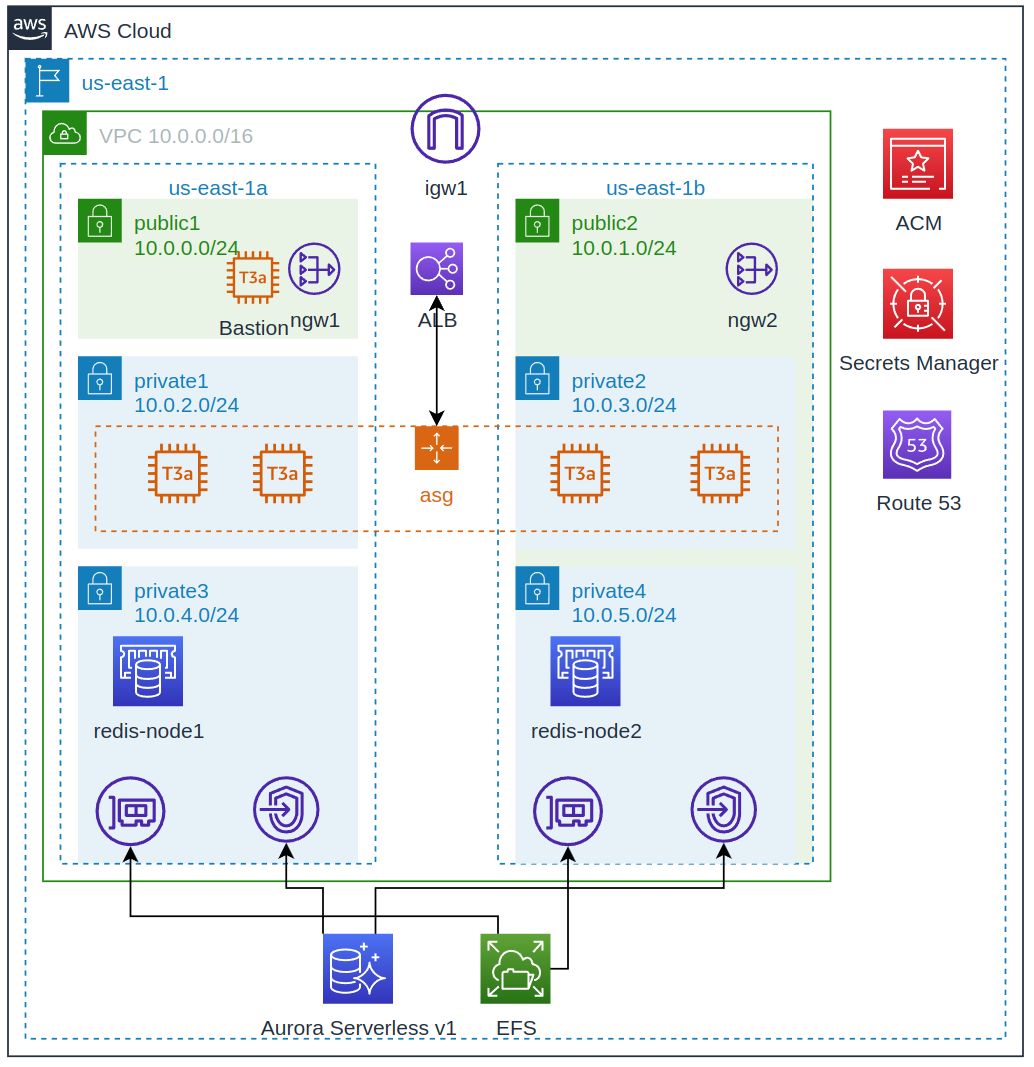
\includegraphics[width=\textwidth]{modul3_architecture.png}
\caption{\label{fig:architecture}Architecture Diagram}
\end{figure}

\section{Task}

\begin{enumerate}
    \item Create VPC with the following specifications:
    \begin{itemize}
        \item IPv4 CIDRs: 10.0.0.0/16
        \item Number of NAT Gateways: 2 
        \begin{enumerate}
            \item Name: ngw1, Subnet: public1
            \item Name: ngw2, Subnet: public2
        \end{enumerate}
        \item Subnets:
        \begin{enumerate}
            \item 
            \begin{itemize}
                \item Subnet Name: public1
                \item IPv4 CIDR block: 10.0.0.0/24
                \item 0.0.0.0/0 is routed to: Internet Gateway
            \end{itemize}
            \vspace{5mm} 
            \item 
            \begin{itemize}
                \item Subnet Name: public2
                \item IPv4 CIDR block: 10.0.1.0/24
                \item 0.0.0.0/0 is routed to: Internet Gateway
            \end{itemize}
            \vspace{5mm} 
            \item 
            \begin{itemize}
                \item Subnet Name: private1
                \item IPv4 CIDR block: 10.0.2.0/24
                \item 0.0.0.0/0 is routed to: NAT Gateway (ngw1) 
            \end{itemize}
            \vspace{5mm} 
            \item 
            \begin{itemize}
                \item Subnet Name: private2
                \item IPv4 CIDR block: 10.0.3.0/24
                \item 0.0.0.0/0 is routed to: NAT Gateway (ngw2) 
            \end{itemize}
            \vspace{5mm} 
            \item 
            \begin{itemize}
                \item Subnet Name: private3
                \item IPv4 CIDR block: 10.0.4.0/24
                \item No additional route.
            \end{itemize}
            \vspace{5mm} 
            \item 
            \begin{itemize}
                \item Subnet Name: private4
                \item IPv4 CIDR block: 10.0.5.0/24
                \item No additional route.
            \end{itemize}
        \end{enumerate}
    \end{itemize}
    \item Create an EC2 key pair.
    \begin{itemize}
        \item Name: lksjabar2022modul3
        \item Key pair type: RSA
        \item Private key file format: .pem
    \end{itemize}
    \item Create a bastion host (EC2 instance) to access resources in private subnet remotely.
        \begin{itemize}
            \item Name: Bastion
            \item OS: Ubuntu 22.04 LTS (HVM)
            \item Subnet: public1
            \item Instance Type: t3a.micro
            \item Public IP Address: Enabled
            \item Security Group Rule: Allow SSH traffic from anywhere
            \item Key pair: lksjabar2022modul3
        \end{itemize}
    \item Create an RDS database with the following specifications:
    \begin{itemize}
        \item Aurora Serverless with PostgreSQL compatibility
        \item Minimum ACU: 0.5
        \item Maximum ACU: 4
        \item Multi-AZ deployment: True
        \item Network Subnet: private3 and private4
    \end{itemize}
    \item Create a database credential on Secrets Manager and attach it to the database
    \item Create ElastiCache with the following specifications:
    \begin{itemize}
        \item Redis Cluster
        \item Enable cluster mode
        \item Enable Multi Availability Zone
        \item Instance Type: t4g.micro
        \item Use default redis port (6379)
        \item Number of shards: 1
        \item Number of replicas: 2
        \item Network Subnet: private3 and private4
    \end{itemize}
    \item Create an EFS file system with the following specifications:
    \begin{itemize}
        \item Storage class: Standard
        \item Transition into IA: 7 days since last access
        \item Transition out of IA: On first access
        \item Performance mode: General Purpose
        \item Throughput mode: Bursting
        \item Encryption: Enable encryption of data at rest
        \item Mount targets:
        \begin{enumerate}
            \item AZ: us-east-1a, Subnet: private3
            \item AZ: us-east-1b, Subnet: private4
        \end{enumerate}
    \end{itemize}
    \item Create an EC2 instance
    \begin{itemize}
        \item Name: InstanceTemplate-modul3
        \item Key pair: lksjabar2022modul3
        \item Instance Type: t3a.micro
        \item Storage: 8 GIB of GP2
        \item Connect to the instance and finish the following instructions inside the instance:
        \begin{itemize}
            \item Clone the application repository from section \ref{resources}. Follow the instruction in README.md to install the application.
            \item Mount the EFS file system to APP\_ROOT/public/images/ where APP\_ROOT is the base directory of the application. Make sure the EFS file system is mounted on startup.
            \item Restart the VM, make sure the application starts on startup.
        \end{itemize}
    \end{itemize}
    \item Create an EC2 Launch Template from InstanceTemplate-modul3 with the following specifications:
    \begin{itemize}
        \item Launch template name: ASG-template-modul3
        \item Key pair: lksjabar2022modul3
        \item Instance Type: t3a.micro
    \end{itemize}
    \item Create Auto Scaling Group with the following specifications:
    \begin{itemize}
        \item Network Subnet: private1 and private2
        \item Load balancing: Attach to a new load balancer
        \begin{itemize}
            \item Load balancer name: ALB-modul3
            \item Load balancer type: Application Load Balancer
            \item Load balancer scheme: Internet-facing
        \end{itemize}
        \item Minimum Capacity: 2
        \item Desired: 2
        \item Max: 6
        \item Scaling policies: Target tracking scaling policy
        \begin{itemize}
            \item Metric type: Average CPU utilization
            \item Target value: 70
        \end{itemize}
    \end{itemize}
    \item Configure ALB-modul3 to redirect HTTP request to HTTPS.
    \item Create a certificate in ACM
    \begin{itemize}
        \item Domain Name: modul3.[YOUR\_DOMAIN]
        \item Validation Method: DNS validation
    \end{itemize}
    \item Add custom domain to the Application Load Balancer
\end{enumerate}
\section{References}\label{references}
\begin{itemize}
\item \href{https://docs.aws.amazon.com/AmazonRDS/latest/AuroraUserGuide/CHAP_AuroraOverview.html}{Amazon Aurora documentation}
\item \href{https://docs.aws.amazon.com/elasticloadbalancing/latest/application/introduction.html}{Application Load Balancer documentation}
\item \href{https://docs.aws.amazon.com/acm/latest/userguide/acm-overview.html}{Certificate Manager documentation}
\item \href{https://docs.aws.amazon.com/efs/latest/ug/whatisefs.html}{EFS documentation}
\item \href{https://docs.aws.amazon.com/AWSEC2/latest/UserGuide/concepts.html}{EC2 documentation}
\item \href{https://docs.aws.amazon.com/autoscaling/ec2/userguide/what-is-amazon-ec2-auto-scaling.html}{EC2 Auto Scaling documentation}
\item \href{https://docs.aws.amazon.com/AmazonElastiCache/latest/red-ug/WhatIs.html}{ElastiCache for Redis documentation}
\item \href{https://docs.aws.amazon.com/Route53/latest/DeveloperGuide/Welcome.html}{Route 53 documentation}
\item \href{https://docs.aws.amazon.com/secretsmanager/latest/userguide/intro.html}{AWS Secrets Manager documentation}
\item \href{https://docs.aws.amazon.com/vpc/latest/userguide/what-is-amazon-vpc.html}{VPC documentation}
\item \href{https://docs.npmjs.com/cli/v8/commands/}{npm documentation}
\item \href{https://classic.yarnpkg.com/en/docs}{yarn documentation}
\item \href{https://pm2.keymetrics.io/docs/usage/process-management/}{PM2 documentation}
\end{itemize}

\section*{Good luck!}

\end{document}